% =====================================================================
%  OASIS 概要设计说明书（Overview Design Document）
%  构建：latexmk -xelatex main.tex    （XeLaTeX + ctex）
% =====================================================================
\documentclass[UTF8,a4paper,11pt]{ctexart}

\usepackage[margin=2.4cm]{geometry}
\usepackage{graphicx}
\usepackage{booktabs}
\usepackage{longtable}
\usepackage{array}
\usepackage{enumitem}
\usepackage{float}
\usepackage{amsmath}
\usepackage{xcolor}
\usepackage[hidelinks]{hyperref}
\usepackage{fancyhdr}

\graphicspath{{figures/}}
\setlist{nosep,leftmargin=2em}

\title{\textbf{OASIS 概要设计说明书}\\[0.4em]
  \large 空间干涉仪观测数据分析与模拟系统\\
  \large Observable Analysis and Simulation for Interferometer-in-Space}
\author{OASIS 设计开发团队}
\date{版本 v0.1（G1 评审稿）\quad 2026-10-10}

\begin{document}
\maketitle

\section*{文档信息}
\addcontentsline{toc}{section}{文档信息}
\begin{center}
\begin{tabular}{>{\bfseries}ll}
\toprule
文档编号 & OASIS-ODD-001 \\
版本 & v0.1（G1 方案设计评审稿） \\
状态 & 提交 G1 评审 \\
编制 & 设计开发（workbench/design） \\
评审 & 评审专家（G1 门禁） \\
依据 & 完成契约 G-001、总计划 PLAN-001 v1.2、科学需求 UR-CAT-001 \\
分发范围 & 四角色工作台面（设计开发 / 科学用户 / 评审专家 / 质量管理） \\
\bottomrule
\end{tabular}
\end{center}

\tableofcontents
\clearpage

\section{引言}

\subsection{目的与范围}

本说明书为 OASIS（空间干涉仪观测数据分析与模拟系统）的概要设计文件，基于已冻结的需求与架构决策基线，
给出系统总体设计、目标层（Targets Layer）的组件级与数据类型级设计，以及各层间接口的权威描述。

\begin{itemize}
  \item \textbf{覆盖范围}：系统 TOP 三层架构（目标层 / 观测量层 / 载荷层）。其中目标层细化到组件与数据类型；
        观测量层与载荷层给出接口级大纲（详细设计待其立项后补充）。
  \item \textbf{不在范围}：OASIS 软件系统的正式实现（约束与假设见第~\ref{sec:constraints} 节）。
  \item \textbf{读者对象}：设计开发、科学用户、评审专家、质量管理人员四类角色。
\end{itemize}

\subsection{术语与缩略语}

\begin{longtable}{>{\raggedright\arraybackslash}p{3.4cm}p{11.5cm}}
\toprule
术语 & 说明 \\
\midrule
\endhead
TOP & Targets--Observables--Payloads：系统级三层架构（目标层 / 观测量层 / 载荷层） \\
目标层 & 观测目标建模：参数化模型 $\rightarrow$ 图像/光谱/光变等可观测模型，并支持参数反演 \\
观测量层 & 干涉观测量（可见度、闭合相位等）的模拟与重建；OIFITS 2 交换的承载层 \\
载荷层 & 仪器数据生成与处理（探测器、条纹、噪声） \\
接口段 / 模型段 / 数据段 & 目标层内部的三段式 V 型纵向架构（层内级，勿与 TOP 三层混淆） \\
\texttt{TargetModel} & 目标层模型抽象基类（含 \texttt{SourceModel}、\texttt{BackgroundModel}、\texttt{TransmissionModel}、\texttt{TargetHistogram}） \\
\texttt{TargetHistogram} & 亮度分布统一容器（图像 / 光谱 / 光变 / 数据立方） \\
\texttt{SpectralModel} / \texttt{SpatialModel} & 光谱 / 空间分布描述符抽象基类 \\
OIFITS 2 & 光学干涉测量数据交换标准 \cite{duvert2017oifits} \\
FITS & 天文图像与表格标准格式 \cite{fits_standard40} \\
WCS & 世界坐标系统（World Coordinate System） \cite{greisen2002wcs} \\
哨兵文件 & 层间异步就绪通知文件：\texttt{.forward\_ready} / \texttt{.inverse\_ready} / \texttt{.error} \\
ADR & 架构决策记录（Architecture Decision Record） \\
ICN & 问题台账条目（Issue/Nonconformity） \\
UR / UC / TV & 科学需求 / 天文用例 / 测试验证报告 \\
G1 / G2 & 阶段门禁：方案设计评审 / 测试报告评审 \\
\bottomrule
\end{longtable}

\subsection{引用文件}

\subsubsection{外部标准与文献}
本说明书引用的标准与文献见文末参考文献，对应关系如下：
OIFITS 2 标准 \cite{duvert2017oifits}；
FITS 4.0 官方标准 \cite{fits_standard40}；
FITS WCS 论文 \cite{greisen2002wcs}；
astropy 科学计算栈 \cite{astropy2022}；
LIFE 空间干涉任务科学评估 \cite{quanz2022life}；
光学干涉测量综述 \cite{monnier2003optical, eisenhauer2023advances}。

\subsubsection{项目内部文件}
\begin{itemize}
  \item \texttt{docs/design/targets.md}：目标层设计开发规范（主规范）；
  \item \texttt{docs/design/targets\_data\_model.md}：目标层数据类型详细设计；
  \item \texttt{docs/design/targets\_interfaces.md}：目标层接口详细设计；
  \item \texttt{docs/design/adr/0001--0007}：架构决策记录（ADR）；
  \item \texttt{workbench/science/requirements/UR-catalog.md}：科学需求集 UR-CAT-001；
  \item \texttt{workbench/PLAN.md}：总计划 PLAN-001；\texttt{workbench/GOAL.md}：完成契约 G-001。
\end{itemize}

\subsection{文档约定}
\begin{itemize}
  \item 代码标识（字段、文件名、命令）采用等宽字体；物理量统一以 \texttt{\{value, unit\}} 表达；
  \item 接口方向以箭头标注：A~$\rightarrow$~B 表示 A 向 B 提供数据；
  \item 文档中的“三段”指目标层内部架构（接口段/模型段/数据段），“三层”指系统级 TOP 架构，两者不可混用。
\end{itemize}

\section{系统概述}

\subsection{科学背景与目标}

OASIS 是一套面向科学用户的空间干涉仪软件工具，目标是帮助科学用户筹划观测任务、分析观测数据；
在工程方案设计与研制阶段，还可用于评估方案科学目标的可实现性，为方案设计及试验验证提供参考。

典型科学场景包括：
\begin{itemize}
  \item \textbf{双星干涉观测}：恒星模型到可见度、闭合相位性质的链路表达；
  \item \textbf{系外行星探测}：LIFE 类空间干涉任务的探测良率评估 \cite{quanz2022life}；
  \item \textbf{AGN / 吸积盘}：多尺度图像与光谱建模；
  \item \textbf{背景与消光}：各向异性背景（黄道光等）与星际消光透过率建模。
\end{itemize}

\subsection{系统功能}

系统包含三大核心功能：

\begin{enumerate}
  \item \textbf{模型全生命周期管理}：统一接收、组织观测目标参数化模型，支持语义解析、冲突检测、
        完整性验证、版本控制与溯源；
  \item \textbf{正向建模与仿真}：由参数化模型生成图像、光谱、光变（偏振预留）可观测模型，
        输出标准 FITS 数据产品；
  \item \textbf{参数反演与模型检验}：从高级科学数据产品中估计模型参数（MCMC / 嵌套采样 / 最大似然），
        开展模型--数据一致性评估。
\end{enumerate}

观测目标模型按五级层级组织：基础模型 $\rightarrow$ 科学主题 $\rightarrow$ 研究方向（可选）
$\rightarrow$ 观测任务 $\rightarrow$ 具体目标，确保基础模型单一来源、通过继承与组合复用。

\subsection{总体架构（TOP 三层）}

\begin{center}
\begin{tabular}{clp{7.2cm}l}
\toprule
层 & 缩写 & 核心职责 & 数据流向 \\
\midrule
\textbf{T} & 目标层 \texttt{targets} & 观测目标建模（图像、光谱、参数）；内部为接口段/模型段/数据段三段式架构 &
目标 $\rightarrow$ 观测量（正演） \\
\textbf{O} & 观测量层 \texttt{observables} & 干涉观测量（可见度、闭合相位）模拟与重建 &
观测量 $\leftrightarrow$ 载荷数据 \\
\textbf{P} & 载荷层 \texttt{payloads} & 仪器数据生成与处理（探测器、条纹、噪声） &
载荷数据 $\rightarrow$ 观测量（反演） \\
\bottomrule
\end{tabular}
\end{center}

\textbf{数据流}：正演（模拟）T $\rightarrow$ O $\rightarrow$ P（目标 $\rightarrow$ 观测量 $\rightarrow$ 载荷数据）；
反演（分析）P $\rightarrow$ O $\rightarrow$ T。

层间数据交换通过文件进行（FITS 家族 + 辅助 JSON/YAML），并以哨兵文件实现异步就绪通知。
目标层内部采用三段式 V 型纵向架构：接口段（面向用户）、模型段（物理计算与统计推断）、
数据段（文件与观测层边界）。

\subsection{用户与角色}

\begin{itemize}
  \item \textbf{科学用户}：提出科学需求（UR），以天文用例开展测试与验证，出局测试报告（TV）；
  \item \textbf{设计开发}：以系统工程方法完成设计与实现工件，出局方案设计报告（DR）；
  \item \textbf{评审专家}：独立评审方案设计报告与测试报告，把控 G1/G2 门禁；
  \item \textbf{质量管理}：过程监督、门禁管理与改进闭环，具叫停权。
\end{itemize}

外部系统：观测量层软件（未来联合部署）、外部天文数据库与文献检索服务。

\subsection{运行环境}

Python $\geq$ 3.12 科学计算栈（numpy、astropy \cite{astropy2022}）；数据交换格式 FITS / OIFITS 2；
文档工程链：XeLaTeX + ctex（本说明书）、PlantUML（设计图）；知识基础设施：OpenAlex（文献检索）与
MinerU（文献全文解析）。计算资源要求详见第~\ref{sec:nonfunctional} 章。

\section{总体设计}

\subsection{设计原则}

\begin{enumerate}
  \item \textbf{格式统一}：尽可能使用 FITS 家族格式（图像 FITS + OIFITS），复用 \texttt{astropy.io.fits} 工具链；
        目标层层间交换以 FITS 为确定格式，HDF5 仅用于开发诊断与大数组缓存；
  \item \textbf{人机友好}：配置类数据采用文本格式；当前版本以 YAML 为确定输入接口；
  \item \textbf{元数据完整}：所有文件携带充分元数据（WCS、时间、仪器状态、版本），保证可追溯；
  \item \textbf{国际兼容}：干涉观测量交换以 OIFITS 2 为核心格式（观测量层 $\leftrightarrow$ 载荷层及对外发布）；
  \item \textbf{异步解耦}：层间通过哨兵文件（\texttt{.forward\_ready} / \texttt{.inverse\_ready}）实现异步就绪通知，
        异常通过 \texttt{.error} 哨兵传递英文错误码与摘要；
  \item \textbf{可插拔、开放式}：观测目标模型按模块独立开发，通过注册机制集成；
  \item \textbf{统一输出接口}：无论何种目标类型，均产出图像、光谱、光变三类标准可观测模型（偏振预留）；
  \item \textbf{段间内存对象契约}：目标层各段之间以与文件格式无关的类型化内存对象交互，
        禁止跨段直接操作字节流或文件句柄；大数组经共享内存视图实现零拷贝传递。
\end{enumerate}

\subsection{数据流}

\begin{itemize}
  \item \textbf{正演链路（T $\rightarrow$ O）}：用户 YAML/API 输入 $\rightarrow$ 接口段校验与提交 $\rightarrow$
        模型段层级解析、冲突检测、完整性验证 $\rightarrow$ 物理引擎生成 \texttt{TargetHistogram}
        $\rightarrow$ 数据段序列化 FITS 输出包 $\rightarrow$ 哨兵 \texttt{.forward\_ready}；
  \item \textbf{反演链路（O $\rightarrow$ T）}：观测层数据产品 + \texttt{.inverse\_ready} $\rightarrow$
        数据段解析为内存对象 $\rightarrow$ 模型段参数估计与统计评估 $\rightarrow$ 接口段呈现科学结论；
  \item \textbf{异步任务生命周期}：排队 $\rightarrow$ 资源准入 $\rightarrow$ 执行 $\rightarrow$ 完成/异常，
        支持资源不足时降级通知（详见第~\ref{sec:targets} 章）。
\end{itemize}

\subsection{外部接口清单}

\begin{center}
\begin{tabular}{p{3.2cm}p{2.2cm}p{2.8cm}p{6.4cm}}
\toprule
接口 & 承载方 & 对端 & 形式与说明 \\
\midrule
用户交互接口 & 接口段 & 科学用户 & YAML 参数化模型 / Python API / CLI；结果报告 JSON/YAML/Markdown/图表 \\
观测量层交换接口 & 数据段 & 观测量层 & FITS 主数据 + JSON/YAML 辅助 + 哨兵文件（异步） \\
本地硬件接口 & Compute Runtime & 本机/集群 & 资源状态采集与发布-订阅推送（计算/存储/网络） \\
\bottomrule
\end{tabular}
\end{center}

\subsection{约束与假设}
\label{sec:constraints}

\begin{itemize}
  \item 当前版本以 \textbf{YAML} 为确定用户输入接口；若未来需要，再增加其它输入途径；
  \item 层间交换以 \textbf{FITS} 为确定格式；HDF5 仅用于诊断与缓存，不参与层间交换；
  \item 观测量层与载荷层尚未立项详细设计，本说明书对其给出接口级大纲；
  \item 本设计阶段的交付不包含 OASIS 软件系统实现；验证以 JSON Schema、YAML 用例样例与检查脚本为载体；
  \item 假设运行环境为 macOS/Linux 工作站（Python $\geq$ 3.12），可扩展至集群（MPI/GPU 为预留能力）；
  \item 观测目标模型的物理语义校验（量纲、非物理取值）由模型段冲突检测承担，不前置到文件解析层。
\end{itemize}

\subsection{需求概述}

科学需求集 UR-CAT-001 共 15 条（必须 9 条 / 应该 6 条），覆盖：模型输入与参数扫描、前向可观测输出、
单位与坐标语义、数据互操作（FITS/OIFITS）、反演估计与一致性评估、背景各向异性、消光建模、
双星与系外行星场景、任务级科学评估、溯源、异步与大文件、错误与可用性。
需求到设计的完整追溯矩阵见第~\ref{sec:traceability} 章。

\section{目标层概要设计}
\label{sec:targets}

\subsection{三段式 V 型纵向架构}

目标层采用三段式 V 字纵向架构，映射“输入 $\rightarrow$ 处理 $\rightarrow$ 输出”的科学工作流：

\begin{itemize}
  \item \textbf{接口段（V 顶）}：OASIS 面向用户及外部系统的唯一外部边界。输入侧通过 CLI、Python API、
        YAML 文件接收参数化模型；输出侧呈现拟合参数、统计一致性评估、不确定性量化与诊断报告。
        不直接处理 FITS 编码或观测量层协议。
  \item \textbf{模型段（V 中）}：核心计算引擎，内设正演与反演双引擎。正演链路将参数化模型经冲突检测、
        完整性验证后，由物理计算生成图像/光谱/光变（偏振预留）的\emph{内存数据结构}；反演链路执行参数估计、
        一致性评估与不确定性量化。本段不感知底层文件格式。
  \item \textbf{数据段（V 底）}：目标层与观测量层的唯一边界。向下游将内存对象序列化为标准 FITS 交付；
        向上游把观测层科学数据产品解析为格式无关的内存对象。目标层内唯有本段感知数据格式与层间协议。
\end{itemize}

\textbf{正演链路}（向下）：用户输入 $\rightarrow$ 接口段 $\rightarrow$ 模型段正演引擎生成可观测模型
$\rightarrow$ 数据段编码为 FITS $\rightarrow$ 观测量层。\textbf{反演链路}（向上）：观测量层数据产品
$\rightarrow$ 数据段解析 $\rightarrow$ 模型段反演与统计评估 $\rightarrow$ 接口段呈现科学结论。

“接口段只应对上、数据段只对下”指职责与接口归属；段间数据流与依赖方向以第~\ref{sec:icd-internal} 节的
接口 A--H 为准：G 为受控横向通道，D/H 等反向回传通过回调与发布-订阅实现，不构成反向依赖。

\begin{figure}[htbp]
  \centering
  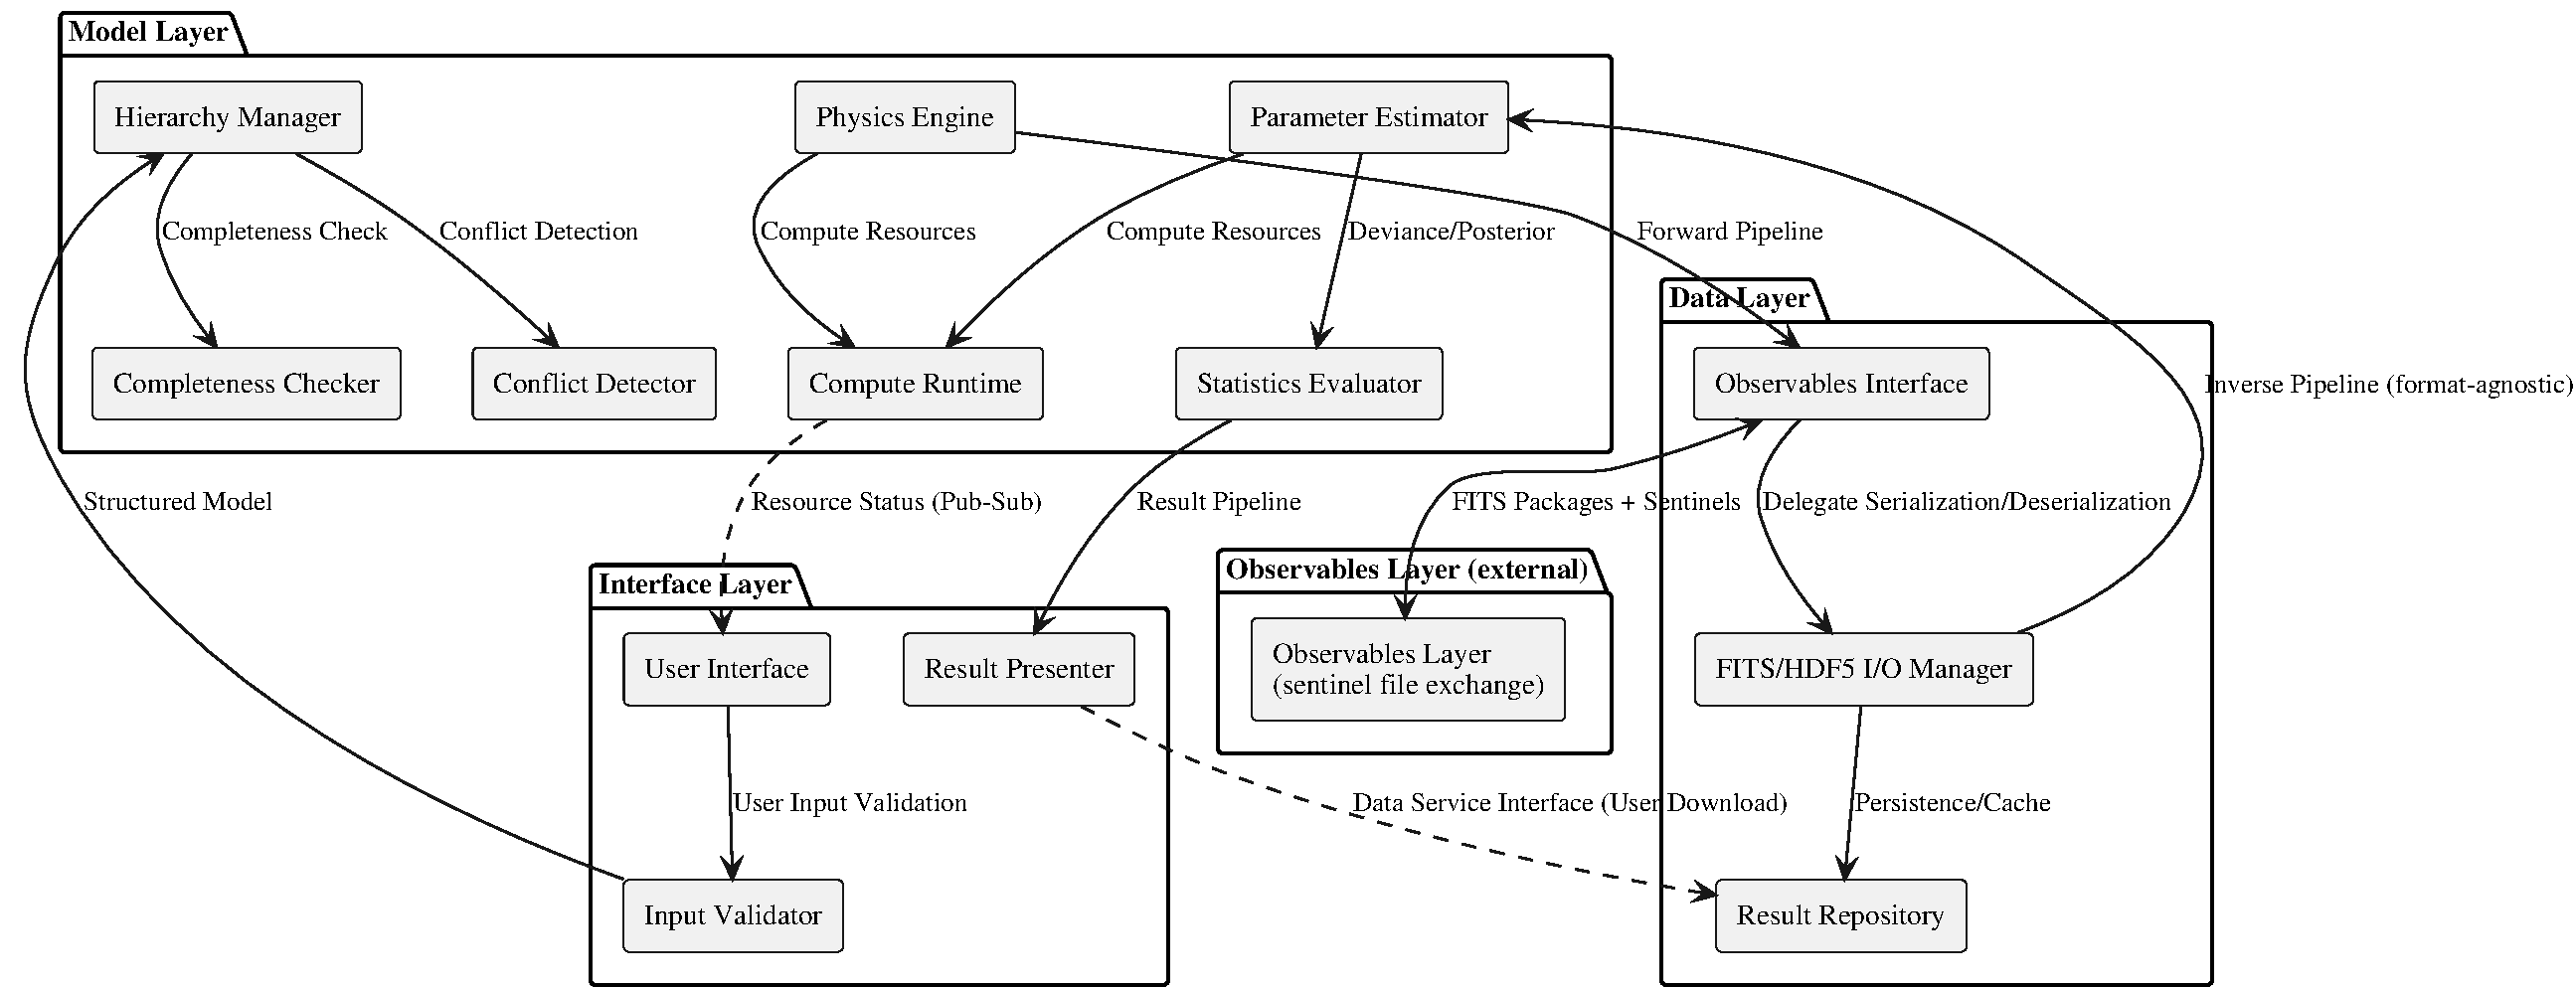
\includegraphics[width=0.98\textwidth]{components.pdf}
  \caption{目标层组件图（含与观测量层的边界）}
  \label{fig:components}
\end{figure}

\subsection{组件职责}

\begin{longtable}{p{4.2cm}p{1.8cm}p{8.8cm}}
\toprule
组件 & 所属段 & 职责摘要 \\
\midrule
\endhead
User Interface & 接口段 & 接收用户输入（CLI/API/自然语言），展示结果与资源状态；唯一外部边界 \\
Input Validator & 接口段 & 语法合法性、字段完整性与数据类型检查（物理语义交由模型段） \\
Hierarchy Manager & 模型段 & 五层级（基础$\rightarrow$主题$\rightarrow$方向$\rightarrow$任务$\rightarrow$目标）继承链管理、版本控制与命名空间隔离 \\
Conflict Detector & 模型段 & 参数物理不自洽、单位制合法性、非物理取值（超光速、负温度等）检测 \\
Completeness Checker & 模型段 & 计算依赖图断点检测，确保参数到可观测体的转换链完整 \\
Physics Engine & 模型段 & 综合源/背景/透过率模型执行数值仿真，生成 \texttt{TargetHistogram} 内存对象 \\
Parameter Estimator & 模型段 & 结合先验执行 MCMC/嵌套采样/最大似然反演，产出后验参数 \\
Statistics Evaluator & 模型段 & 偏离度（$\chi^2$、残差）、置信区间、模型选择准则与一致性评估 \\
Compute Runtime & 模型段 & 并行调度、异构计算、缓存管理、资源监视与准入评估 \\
Result Presenter & 接口段 & 生成用户级报告（JSON/YAML/Markdown/图表）；不编辑 FITS \\
Observables Interface & 数据段 & 层间交换目录管理、哨兵文件通知、正演/反演文件包组织 \\
FITS/HDF5 I/O Manager & 数据段 & FITS 序列化/反序列化（WCS 与元数据）；向上交付格式无关内存对象 \\
Result Repository & 数据段 & 持久化、缓存、版本快照与生命周期管理 \\
\bottomrule
\end{longtable}

\subsection{核心数据结构}

\begin{figure}[htbp]
  \centering
  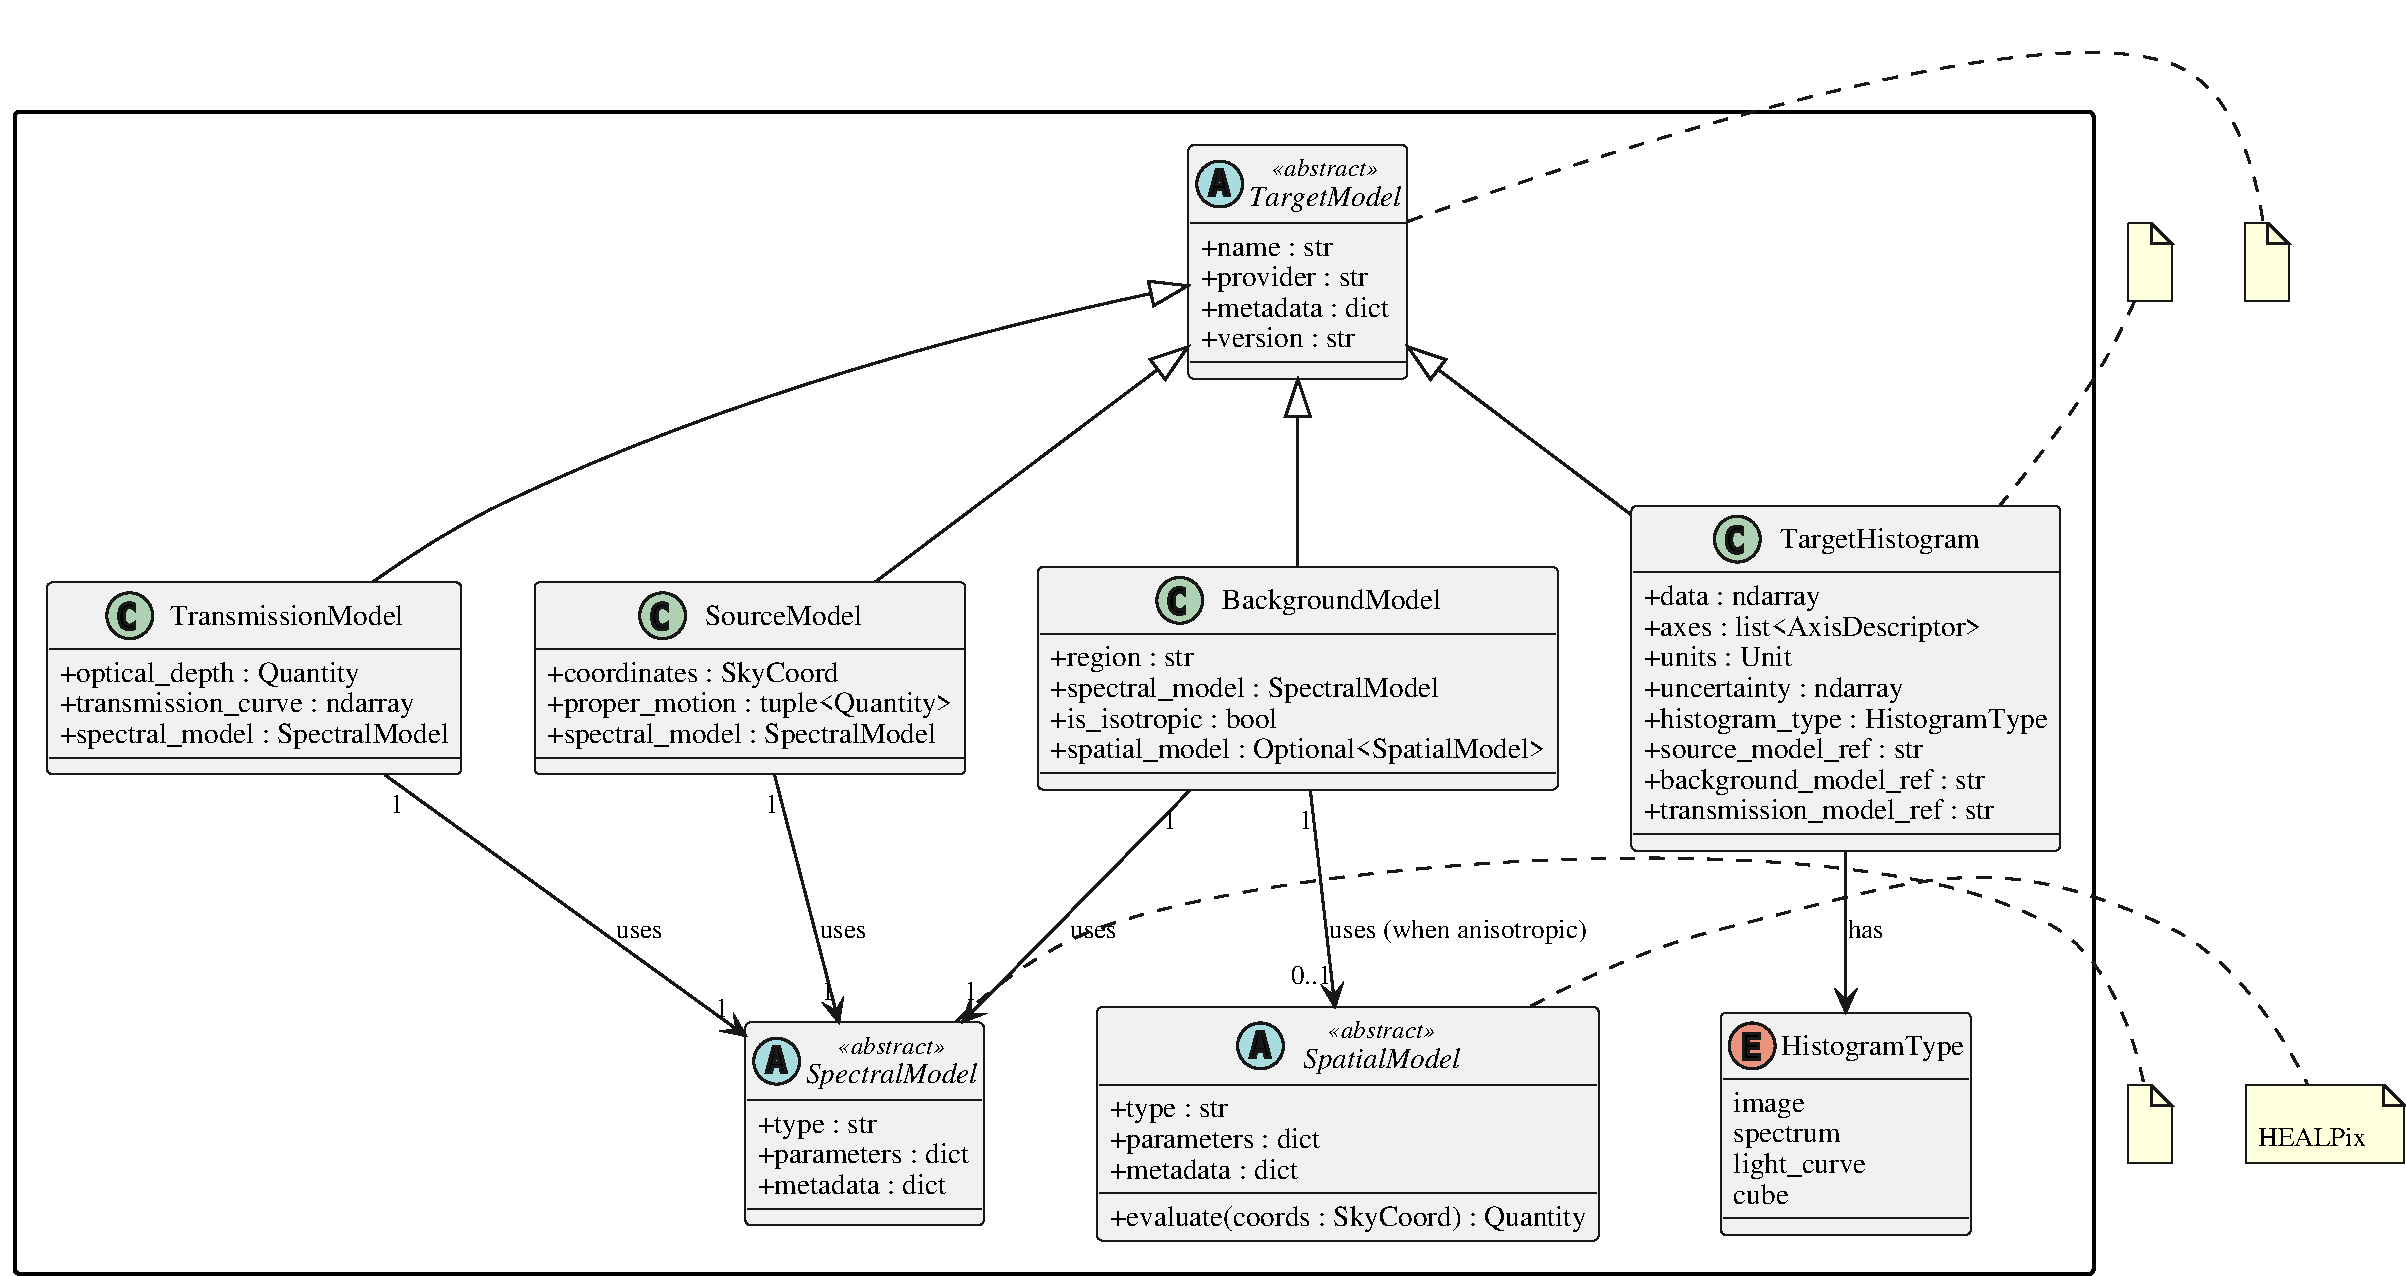
\includegraphics[width=\textwidth]{classes.pdf}
  \caption{目标层核心类图}
  \label{fig:classes}
\end{figure}

\begin{itemize}
  \item \texttt{TargetModel}：抽象基类，字段 \texttt{name} / \texttt{provider} / \texttt{version} /
        \texttt{metadata} / \texttt{hierarchy}；模型实例视为逻辑不可变，变更须递增版本。
  \item \texttt{SourceModel}：\texttt{coordinates}（SkyCoord 兼容）、\texttt{proper\_motion}、
        \texttt{spectral\_model}；\texttt{epoch}/\texttt{frame}（默认 J2000/ICRS）与可选星表块
        \texttt{catalogue}（ID/视差/测光，ADR 0009）。
  \item \texttt{DynamicalModel}（ADR 0008）：定位太阳系天体（小行星等）——\texttt{epoch}、
        \texttt{elements}（\texttt{a}/\texttt{e}/\texttt{i}/\texttt{raan}/\texttt{argp} 与 \texttt{M} 或 \texttt{Tp}）、
        \texttt{H}、可选 \texttt{category} 与位置快照序列；位置计算属物理引擎实现阶段。
  \item \texttt{BackgroundModel}：\texttt{region}、\texttt{spectral\_model}、\texttt{is\_isotropic}（默认 true）、
        \texttt{spatial\_model}（各向异性时必填，见 ADR 0006）。
  \item \texttt{TransmissionModel}：\texttt{optical\_depth}、\texttt{transmission\_curve}（可选，优先于参数化模型）、
        \texttt{spectral\_model}。
  \item \texttt{TargetHistogram}：统一亮度分布容器——\texttt{data}、\texttt{axes}、\texttt{units}、
        \texttt{uncertainty}、\texttt{histogram\_type}（image / spectrum / light\_curve / cube）与三个
        模型引用字段（源/背景/透过率），支持正演溯源与反演回写。
  \item \texttt{SpectralModel} / \texttt{SpatialModel}：对称的抽象描述符（\texttt{type} / \texttt{parameters} /
        \texttt{metadata}）；\texttt{SpatialModel.evaluate(coords)} 返回归一化或绝对亮度。
  \item 枚举：\texttt{HistogramType}、\texttt{AxisType}（spatial / spectral / temporal / other）。
  \item 关键不变量（节选）：\texttt{axes} 长度等于 \texttt{data.ndim}；\texttt{uncertainty} 与 \texttt{data}
        形状一致；\texttt{is\_isotropic=False} 时 \texttt{spatial\_model} 必填。
\end{itemize}

\subsection{内部接口（A--H）}
\label{sec:icd-internal}

段间接口遵循\emph{内存对象契约}：一律通过类型化、与文件格式无关的抽象数据交互；大数组经共享内存视图零拷贝传递。

\begin{longtable}{p{2.6cm}p{3.2cm}p{3.0cm}p{5.8cm}}
\toprule
接口 & 方向 & 实现途径 & 要点 \\
\midrule
\endhead
A 输入管道 & 接口段 $\rightarrow$ 模型段 & 函数调用（结构化内存对象） & 参数化模型、单位制声明、任务上下文与模式标识 \\
B 正演管道 & 模型段 $\rightarrow$ 数据段 & 共享内存视图 & \texttt{TargetHistogram} 大数组句柄，零拷贝写入 \\
C 反演管道 & 数据段 $\rightarrow$ 模型段 & 共享内存视图 & 解析后的科学数据产品、噪声与质量标记 \\
D 结果管道 & 模型段 $\rightarrow$ 接口段 & 函数调用 / 回调 & 拟合参数、统计量、诊断数据（禁止外部文件传输） \\
E 计算支撑 & 模型段 $\leftrightarrow$ Compute Runtime & 消息队列 + 共享内存句柄 & 任务描述、资源调度状态、缓存命中 \\
F 持久化支撑 & 数据段 $\leftrightarrow$ 结果仓库 & 进程内函数调用 & 存储/检索、缓存与生命周期（段内耦合） \\
G 数据服务 & 接口段 $\rightarrow$ 数据段（受控横向） & 请求-响应端口（Unix Domain Socket） & 用户级数据下载；禁止绕行模型段做科学计算交换 \\
H 资源状态 & 模型段 $\rightarrow$ 接口段 & 发布-订阅事件流 & 资源状态与准入评估推送（含降级建议） \\
\bottomrule
\end{longtable}

段间诊断导出（JSON/HDF5 文件）为受控补充途径，仅用于开发、测试与故障诊断，生产环境默认禁用。

\subsection{关键流程}

\begin{figure}[H]
  \centering
  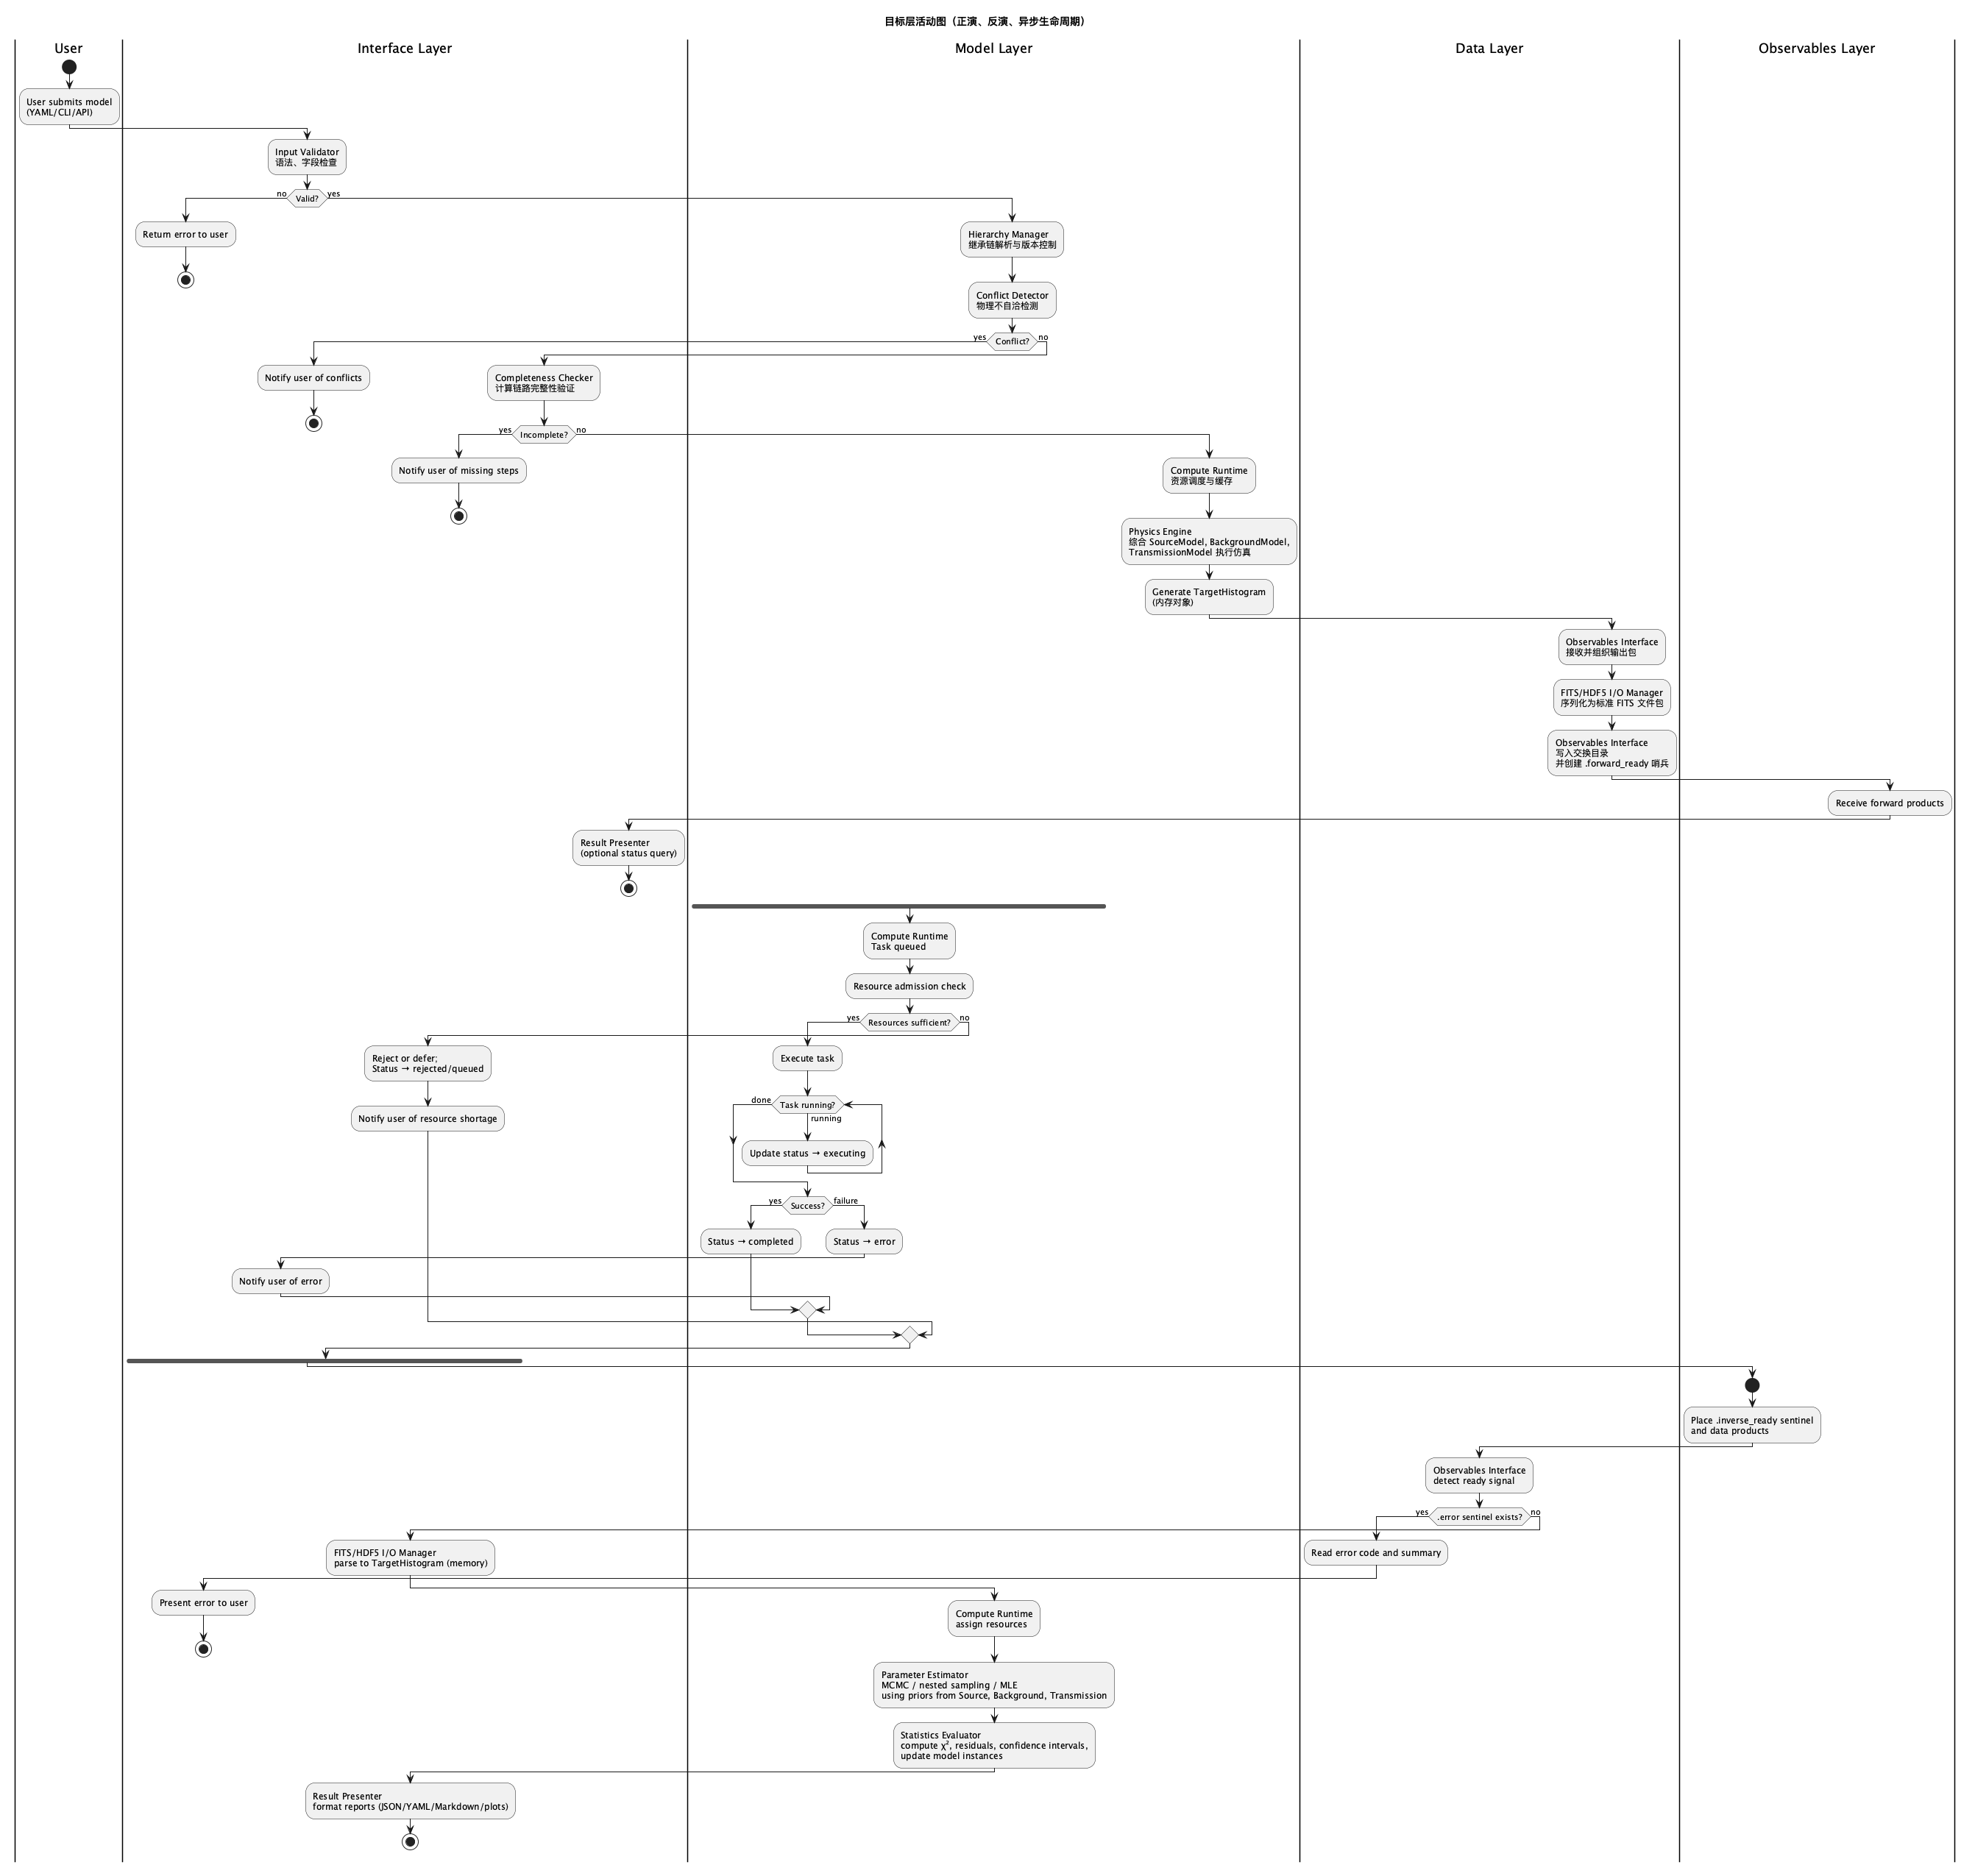
\includegraphics[width=\textwidth,height=0.82\textheight,keepaspectratio]{activities.png}
  \caption{目标层活动图（正演、反演与异步任务生命周期）}
  \label{fig:activities}
\end{figure}

\begin{itemize}
  \item \textbf{正演}：User Interface $\rightarrow$ Input Validator $\rightarrow$ Hierarchy Manager
        （冲突/完整性检测）$\rightarrow$ Compute Runtime 调度 $\rightarrow$ Physics Engine 仿真 $\rightarrow$
        \texttt{TargetHistogram} $\rightarrow$ Observables Interface $\rightarrow$ FITS I/O 序列化 $\rightarrow$
        交换目录 + \texttt{.forward\_ready} 哨兵。
  \item \textbf{反演}：\texttt{.inverse\_ready} 触发 $\rightarrow$ Observables Interface 检测 $\rightarrow$
        FITS I/O 解析为内存对象 $\rightarrow$ Parameter Estimator（结合先验）$\rightarrow$ Statistics Evaluator
        $\rightarrow$ Result Presenter 呈现报告。
  \item \textbf{异步生命周期与容错}：任务排队 $\rightarrow$ 资源准入（不足时拒绝/降级并通知）$\rightarrow$
        执行 $\rightarrow$ 完成/异常；观测层交换失败时读取 \texttt{.error} 错误码向上传播。
\end{itemize}

\section{观测量层与载荷层概要（接口级大纲）}
\label{sec:layers}

观测量层与载荷层的详细设计待其立项后补充；本章给出与目标层及相互之间已确定的接口级约束。

\subsection{观测量层}

\begin{itemize}
  \item \textbf{职责}：干涉观测量（可见度振幅/相位、闭合相位等）的模拟与重建。
  \item \textbf{数据交换}：以 OIFITS 2 \cite{duvert2017oifits} 为核心格式；$(u,v)$ 采样点内嵌于 OIFITS 表的
        \texttt{UCOORD}、\texttt{VCOORD} 列，无需单独文件；干涉仪动态状态（延迟线位置、环境参数、指向修正）
        以 JSON 辅助文件与 OIFITS 配套保存。
  \item \textbf{与目标层的接口}：接收目标层正演产品包（FITS 图像/光谱/光变；见第~\ref{sec:formats} 章）；
        向目标层提供反演输入包（携带 \texttt{DATA\_QUAL} 数据质量标记、仪器标识与校准版本）并以
        \texttt{.inverse\_ready} 哨兵通知就绪；处理失败时放置 \texttt{.error} 文件（错误码与英文摘要）。
  \item \textbf{对外兼容}：与国内外干涉数据处理工具集（如 JMMC 工具链）以 OIFITS 2 互操作。
\end{itemize}

\subsection{载荷层}

\begin{itemize}
  \item \textbf{职责}：仪器数据生成与处理（探测器、条纹、噪声）。
  \item \textbf{数据}：原始条纹数据（自定义二进制或 FITS）；工程辅助数据（望远镜指向、活塞误差、环境监测）
        以 OIFITS 自定义扩展表 \texttt{OI\_ENG} / \texttt{OI\_ENV} 承载，确保时间同步；
        经条纹提取与校准后的干涉采样输出为标准 OIFITS 2，供观测量层进一步分析。
\end{itemize}

\subsection{后续工作}

\begin{itemize}
  \item 两层详细设计（组件、文件与表结构清单、校验规则）待立项后编制；
  \item OIFITS 2 表结构清单与校验工具、与 JMMC 工具集的互操作测试纳入后续验证计划；
  \item 目标层侧接口（数据段）已冻结：层间交换为 FITS 主数据 + JSON/YAML 辅助 + 哨兵协议，
        对接两层不需要目标层设计变更。
\end{itemize}

\section{数据与文件格式}
\label{sec:formats}

\subsection{用户输入：YAML 参数化模型}

顶层字段与约束：
\begin{itemize}
  \item 必填：\texttt{oasis\_version}、\texttt{theme}，以及至少一个模型定义块（\texttt{source} 必选；
        \texttt{background}、\texttt{transmission} 可选）；编码 UTF-8；
  \item 物理量统一以 \texttt{\{value, unit\}} 表达，单位兼容天文标准单位制；
  \item \texttt{extends} 支持引用基础模型或上级主题；参数扫描支持 \texttt{linspace} / \texttt{logspace} / \texttt{list}；
  \item 物理语义校验（量纲一致性、非物理取值）由模型段执行，不前置在文件解析层。
\end{itemize}

示例（节选）：
\begin{verbatim}
oasis_version: "1.0"
theme: "stellar"
source:
  name: "sun_like_1"
  extends: "stellar_base"
  coordinates:
    ra: {value: 83.633, unit: "deg"}
    dec: {value: 22.014, unit: "deg"}
    distance: {value: 10, unit: "pc"}
  proper_motion:
    pm_ra_cosdec: {value: 34.5, unit: "mas/yr"}
    pm_dec: {value: -12.3, unit: "mas/yr"}
  spectral_model:
    type: "blackbody"
    parameters:
      temperature: {value: 5778, unit: "K"}
transmission:
  name: "ism_extinction"
  optical_depth: {value: 0.3, unit: ""}
  spectral_model:
    type: "power_law"
    parameters:
      alpha: {value: -1.5, unit: ""}
      reference_wavelength: {value: 5500, unit: "angstrom"}
\end{verbatim}

\subsection{正演输出包（目标层 $\rightarrow$ observables）}

\begin{itemize}
  \item \textbf{主 FITS}：\texttt{TargetHistogram} 序列化（二维/三维/四维数组），WCS 完备自洽，
        光变曲线含时间轴描述；
  \item \textbf{必填头关键字}：\texttt{OASIS\_VER}、\texttt{MODEL\_ID}、\texttt{TIMESTAMP}、
        \texttt{TARGET\_CLASS}、\texttt{OASIS\_OBS\_INTF\_VER}，以及 \texttt{SRC\_MODEL} /
        \texttt{BKG\_MODEL} / \texttt{TRANS\_MODEL} / \texttt{SPATIAL\_TYP}（无对应内容时为空字符串）；
  \item \textbf{辅助文件}：\texttt{params.json}（参数侧写）、\texttt{config.yaml}（观测配置摘要）、
        \texttt{processing\_log.txt}（计算过程日志）；CSV/TSV 处理指令可选；
  \item \textbf{哨兵}：全部写入完成后生成 \texttt{.forward\_ready}。
\end{itemize}

\subsection{反演输入包（observables $\rightarrow$ 目标层）}

\begin{itemize}
  \item \textbf{主 FITS}：科学数据产品，结构与正演输出一致（\texttt{TargetHistogram} 存储形态）；
  \item \textbf{头关键字}：\texttt{TASK\_ID}、\texttt{INSTRUMENT}、\texttt{CALIB\_VER}、\texttt{DATA\_QUAL}
        （good / warning / bad）、\texttt{OASIS\_OBS\_INTF\_VER}；
  \item \textbf{辅助文件}：\texttt{noise\_model.json}（噪声模型）、\texttt{observation\_config.yaml}
        （观测配置）、\texttt{instrument\_response.json}（仪器响应，可选）；
  \item \textbf{哨兵}：\texttt{.inverse\_ready}；
  \item \textbf{异常路径}：\texttt{.error} 文件承载 JSON 载荷（\texttt{error\_code} / \texttt{english\_message} /
        \texttt{timestamp}），错误码统一为 \texttt{E\_\{DOMAIN\}\_\{CODE\}} 格式（如 \texttt{E\_OBS\_001}）。
\end{itemize}

\subsection{哨兵协议}

\begin{center}
\begin{tabular}{lll}
\toprule
哨兵文件 & 放置方 & 含义 \\
\midrule
\texttt{.forward\_ready} & 目标层 & 正演产物就绪，observables 层可消费 \\
\texttt{.inverse\_ready} & observables 层 & 反演输入数据就绪 \\
\texttt{.error} & 任意方 & 处理失败，阻止后续自动流转 \\
\bottomrule
\end{tabular}
\end{center}

\subsection{与 OIFITS 2 的关系}

目标层与 observables 层之间交换的是目标区域的亮度分布产品（图像/光谱/光变），以 FITS 主数据 +
JSON/YAML 辅助文件表达，\emph{不使用 OIFITS 表结构}。OIFITS 2 是干涉观测量（可见度、闭合相位等）的交换标准，
适用于观测量层与载荷层之间及对外发布环节；当观测流程需要将目标模型转换为干涉观测量时，
由观测量层负责 OIFITS 封装，目标层不直接产出 OIFITS。

\section{非功能设计}
\label{sec:nonfunctional}

\subsection{性能}

\begin{itemize}
  \item \textbf{交互侧}：交互式操作低延迟响应；任务提交支持高吞吐（批量任务与蒙特卡洛场景）；
        结果返回支持分页、流式传输与增量更新；资源状态查询低延迟，不阻塞交互；
  \item \textbf{数据交换}：支持大体积科学数据的高效传输与并发任务的严格数据隔离；
        序列化/反序列化性能匹配观测模拟与分析的实时性要求；
  \item \textbf{计算}：段间大数组以共享内存视图零拷贝传递；缓存基于参数哈希（LRU）避免重复计算；
        支持 CPU/GPU 异构与 MPI 分布式调度的扩展能力；
  \item \textbf{资源探测}：网络、计算、存储状态采集须低开销，不挤占科学计算与传输带宽。
\end{itemize}

\subsection{可靠性}

\begin{itemize}
  \item 异步任务生命周期：排队 $\rightarrow$ 资源准入 $\rightarrow$ 执行 $\rightarrow$ 完成/异常，
        状态可查询、事件可订阅；
  \item 层间容错：哨兵文件驱动解耦；\texttt{.error} 哨兵携带英文错误码与摘要，向上传播不静默失败；
        长链路任务支持重试；
  \item 资源不足时执行排队、拒绝或降级策略并向用户提示，避免阻塞观测任务时效性；
  \item 缓存与版本一致性检查，防止陈旧结果复用。
\end{itemize}

\subsection{安全与数据保护}

\begin{itemize}
  \item 用户数据下载经接口 G（受控 Unix Domain Socket 端口），禁止接口段直接穿透底层存储句柄；
  \item 数据访问权限控制与生命周期管理，防止未授权访问；
  \item 段间诊断导出（JSON/HDF5）仅限开发/测试/故障诊断，生产环境默认禁用；
        组件内部诊断文件须命名空间隔离，禁止写入层间交换目录、结果仓库与用户工作区。
\end{itemize}

\subsection{可维护性与文档工程}

\begin{itemize}
  \item \textbf{单一来源原则}：设计规范描述“是什么”，ADR 记录“为什么”；术语与字段跨文档一致；
  \item \textbf{版本策略}：外部接口（YAML schema、FITS 关键字）以 \texttt{oasis\_version} 标识；
        内部模型以 \texttt{model\_version} 管理变迁；事件主题携带主版本（如 \texttt{oasis.v1.*}）；
  \item \textbf{需求—设计—验证追溯}：UR $\rightarrow$ 设计落点 $\rightarrow$ UC/TV 全链可追溯（第~\ref{sec:traceability} 章）；
  \item \textbf{验证工件}：JSON Schema、YAML 用例样例与一致性检查脚本纳入交付与回归。
\end{itemize}

\section{接口控制摘要}
\label{sec:icd-summary}

\subsection{错误码}

统一错误码格式 \texttt{E\_\{DOMAIN\}\_\{CODE\}}，附英文摘要；由 Result Presenter 封装进结果报告呈现。

\begin{center}
\begin{tabular}{ll}
\toprule
错误码 & 说明 \\
\midrule
\texttt{E\_INPUT\_001} & YAML syntax error \\
\texttt{E\_INPUT\_002} & Missing required field \\
\texttt{E\_INPUT\_003} & Invalid unit string \\
\texttt{E\_COMPUTE\_001} & Insufficient memory \\
\texttt{E\_COMPUTE\_002} & Parameter out of physical bounds \\
\texttt{E\_COMPUTE\_003} & Simulation diverged \\
\texttt{E\_DATA\_001} & FITS header incompatible \\
\texttt{E\_DATA\_002} & .error sentinel received from observables \\
\texttt{E\_OBS\_001} & Observables layer processing failed（校准、条纹提取等） \\
\texttt{E\_COMM\_001} & Observatory node unreachable \\
\bottomrule
\end{tabular}
\end{center}

\subsection{任务状态枚举}

\begin{center}
\begin{tabular}{ll}
\toprule
枚举值 & 含义 \\
\midrule
\texttt{queued} & 已提交排队 \\
\texttt{resource\_wait} & 等待资源准入 \\
\texttt{running} & 执行中 \\
\texttt{completed} & 正常完成 \\
\texttt{failed} & 异常终止 \\
\texttt{cancelled} & 已取消 \\
\bottomrule
\end{tabular}
\end{center}

\subsection{事件主题}

\begin{itemize}
  \item 资源状态：\texttt{oasis.resource.status}（发布-订阅；接口段订阅用于系统健康展示与任务降级）；
  \item 任务状态：\texttt{oasis.task.\{task\_id\}}，载荷示例：
\end{itemize}

\begin{verbatim}
{
  "task_id": "...",
  "old_state": "queued",
  "new_state": "running",
  "timestamp": "...",
  "message": "Starting physics simulation"
}
\end{verbatim}

\subsection{版本控制}

\begin{itemize}
  \item 外部接口以 \texttt{oasis\_version}（YAML）与 \texttt{OASIS\_OBS\_INTF\_VER}（FITS 头）标识；
  \item 内部 Pydantic 模型以类级 \texttt{model\_version} 管理变迁，主版本不兼容变更须保留旧解析器至少一个版本周期；
  \item 发布-订阅主题命名含主版本以支持多版本共存。
\end{itemize}

\section{需求追溯与验证}
\label{sec:traceability}

\subsection{需求—设计追溯矩阵}

科学需求集 UR-CAT-001（15 条：必须 9 / 应该 6）到本说明书设计的追溯如下
（“覆盖”指设计层面已给出承载点；用例级验证见第~\ref{sec:traceability} 章后续小节与 TV 报告）。

\begin{longtable}{p{1.5cm}p{4.6cm}p{6.0cm}p{2.6cm}}
\toprule
UR & 需求摘要 & 设计落点（本说明书） & 状态 \\
\midrule
\endhead
UR-001 & 目标建模 YAML 输入（源必选，背景/透过率可选） & 第~6.1 节；第~4.3 节数据模型 & 覆盖 \\
UR-002 & 参数扫描（linspace/logspace/list） & 第~6.1 节 & 覆盖 \\
UR-003 & 前向可观测输出（图像/光谱/光变，偏振预留） & 第~4.3、4.5 节 & 覆盖 \\
UR-004 & 单位与坐标语义（\{value,unit\}；SkyCoord/ICRS） & 第~4.3 节；第~6.1 节 & 覆盖 \\
UR-005 & 数据互操作（FITS/WCS；OIFITS 对齐） & 第~6.2--6.5 节 & 覆盖 \\
UR-006 & 反演参数估计（MCMC/嵌套采样/MLE） & 第~4.2、4.5 节 & 覆盖 \\
UR-007 & 一致性评估（$\chi^2$/残差/AIC/BIC/贝叶斯因子） & 第~4.2、4.5 节 & 覆盖 \\
UR-008 & 背景各向异性（空间模型，黄道光等） & 第~4.3 节；ADR 0006 & 覆盖 \\
UR-009 & 消光/透过率（幂律/透过率曲线） & 第~4.3 节 & 覆盖 \\
UR-010 & 双星场景（可见度/闭合相位链路） & 第~4.3 节 + 第~5.1 节接口 & 覆盖（接口级） \\
UR-011 & 系外行星（凌星光变 + 光谱） & 第~4.3 节 & 覆盖 \\
UR-012 & 任务级科学评估输入（LIFE 类） & 第~2.1--2.2 节 & 覆盖（接口级） \\
UR-013 & 溯源（模型引用字段/版本） & 第~4.3 节；第~6.2 节 & 覆盖 \\
UR-014 & 异步与大文件（哨兵/GB 级） & 第~4.5、7.1--7.2 节 & 覆盖 \\
UR-015 & 错误与可用性（英文错误码/状态查询） & 第~8.1--8.3 节 & 覆盖 \\
\bottomrule
\end{longtable}

\subsection{验证计划（摘要）}

\begin{itemize}
  \item \textbf{文档一致性}（E1--E4）：死链 0、术语/字段一致、YAML 示例经 JSON Schema 校验，
        由验证脚本 \texttt{workbench/design/verify.sh} 统一执行；
  \item \textbf{交付构建}（E5--E6）：本说明书经 \texttt{latexmk -xelatex} 编译通过；引用文献库 key；
  \item \textbf{过程闭环}（E7--E9）：ICN 台账 0 OPEN（A 级经独立复核关闭）；
        G1/G2 评审记录（RR/GR）与测试报告（TV）齐备且结论为通过。
\end{itemize}

\subsection{天文用例概览（P4 测试覆盖）}

\begin{center}
\begin{tabular}{lll}
\toprule
用例 & 场景 & 观测要点 \\
\midrule
UC-1 & 双星干涉观测 & 几何参数到可见度/闭合相位的预期 \\
UC-2 & 系外行星场景 & 凌星光变 + 光谱组合模型 \\
UC-3 & AGN / 吸积盘 & 多尺度图像 + 光谱 \\
UC-4 & 消光与各向异性背景 & TransmissionModel + BackgroundModel 组合 \\
UC-5 & 参数扫描与正反演闭环 & YAML 扫描输入 $\rightarrow$ 反演输入包 $\rightarrow$ 参数更新 \\
\bottomrule
\end{tabular}
\end{center}

用例的正式条目（输入样例、预期结果、通过判据）与实测记录见 \texttt{science/use-cases/} 与
\texttt{science/test-reports/TV-001}（P4 阶段产出）。

\section{附录}

\subsection{架构决策记录（ADR）索引}

\begin{center}
\begin{tabular}{lll}
\toprule
编号 & 标题 & 状态 \\
\midrule
ADR 0001 & 采用架构决策记录机制 & 已接受 \\
ADR 0002 & 目标层采用三段式 V 型纵向架构 & 已接受 \\
ADR 0003 & 建立核心参数化模型层次结构 & 已接受 \\
ADR 0004 & 统一分布表示为 TargetHistogram & 已接受 \\
ADR 0005 & 将 TargetModel 溯源字段命名为 provider & 已接受 \\
ADR 0006 & 为 BackgroundModel 增加空间各向异性支持 & 已接受 \\
ADR 0007 & TargetModel 基类字段设计 & 已接受 \\
\bottomrule
\end{tabular}
\end{center}

\subsection{文档变更记录}

\begin{center}
\begin{tabular}{llp{8.2cm}}
\toprule
版本 & 日期 & 说明 \\
\midrule
v0.1 & 2026-10-10 & 初版（G1 评审稿）：基于清理后的文档基线（ICN 台账 0 OPEN）编制 \\
\bottomrule
\end{tabular}
\end{center}

\subsection{配套文件清单}

\begin{itemize}
  \item 设计基线：\texttt{docs/design/targets.md}、\texttt{targets\_data\_model.md}、\texttt{targets\_interfaces.md}；
  \item 架构决策：\texttt{docs/design/adr/0001--0007}；
  \item 设计图（PlantUML 源）：\texttt{docs/diagrams/targets/\{classes,components,activities\}.puml}；
  \item 科学需求：\texttt{workbench/science/requirements/UR-catalog.md}（UR-CAT-001）；
  \item 文献库：\texttt{workbench/library/}（登记册、BibTeX 与全文解析；本说明书参考文献取自其中 key）。
\end{itemize}


% 参考文献（文献库 key，见 workbench/library/registry.md）
\nocite{duvert2017oifits,fits_standard40,greisen2002wcs,astropy2022,quanz2022life,monnier2003optical,eisenhauer2023advances}
\bibliographystyle{plain}
\bibliography{refs}

\end{document}
